\documentclass[11pt,a4paper]{article}

\usepackage[left=2cm,text={17cm,24cm},top=3cm]{geometry}
\usepackage[slovak]{babel}
\usepackage[utf8]{inputenc}
\usepackage[T1]{fontenc}

\usepackage{url}
\usepackage{enumerate}

\usepackage{float}
\usepackage{xcolor}
\usepackage{siunitx}
\usepackage{amsmath}
\usepackage{accents}
\usepackage{listings}
\usepackage{csquotes}
\usepackage{hyperref}
\usepackage{textcomp}
\usepackage{amsfonts}
\usepackage{breakurl}
\usepackage{etoolbox}
\usepackage{graphicx}
\usepackage{multicol}
\usepackage{multirow}
\usepackage{supertabular}
\usepackage{tikz}
\usepackage[titles]{tocloft}

\renewcommand{\cftdot}{}
\newcommand{\red}[1]{\textcolor{red}{#1}}
\newcommand{\blue}[1]{\textcolor{blue}{#1}}

\definecolor{OliveGreen}{rgb}{0,0.7,0}
\newcommand{\green}[1]{\textcolor{OliveGreen}{#1}}

\setlength\parindent{0pt}

\def\UrlBreaks{\do\/\do-}
\newcommand{\tilda}{\raisebox{0.5ex}{\texttildelow}}

\graphicspath{{.}}
\patchcmd{\thebibliography}{\section*{\refname}}{}{}{}

\begin{document}

\begin{titlepage}
    \begin{center}
        \Huge
        \textsc{
            Fakulta informačních technologií\\
            Vysoké učení technické v~Brně
        }
        \vspace{80px}
        \begin{figure}[!h]
            \centering
            
\includegraphics[scale=0.3]{img/vutbr-fit-logo.eps}
        \end{figure}
        \\[15mm]
        \Huge{
            \textbf{
                TIN
            }
        }
        \\[1.5mm]
        \huge{
            \textbf{
                Teoretická informatika
            }
        }
        \\[2.5em]
        \LARGE{
            \textbf{
                2. domáca úloha
            }
        }
        \vfill
    \end{center}
        \Large{
            Adrián Tóth (xtotha01)\hfill \today
        }
\end{titlepage}

\setlength{\parskip}{0pt}
\hypersetup{hidelinks}\tableofcontents
\setlength{\parskip}{0pt}


\newpage
\section{Príklad číslo 1} %############################################################################

\subsection{(a)}\label{sec:a}

\textit{Definice 4.29}~\cite{TIN}(str. č. 97) Označme $ZAV_n$ pre $n \geq 0$ jazyky setávající ze všech vyvážených řetězců závorek $n$ typů. Tyto jazyky -- označované též jako Dyckovy jazyky -- jsou generovány gramatikami s pravidly tvaru: $S \rightarrow [^{1}\ S\ ]^{1} \ |\  [^{2}\ S\ ]^{2} \ |\  ... \ |\  [^{n}\ S\ ]^{n} | \ SS \ | \ \varepsilon $

\rule{17cm}{0.4pt}

\hfill\\[-2em]

Z hore uvedenej definície pre náš príklad vyplýva, že náš Dyckov jazyk $L$ je generovaný gramatikou $G_{D}$, definovanou ako $G_{D} = (\{S'\},\{[,]\},P,S')$ kde množina prepisovacích pravidiel $P$ je daná ako

\begin{center}
$S' \rightarrow \varepsilon \ | \ S'S' \ | \ [\ S' \ ]$
\end{center}

ktorá obsahuje iba jeden typ zátvoriek ktorými sú $[$ a $]$.\\

Pre každé slovo $w \in L$, pre ktoré platí že $w \neq \varepsilon$, muselo byť aspoň raz použité pravidlo $S' \rightarrow [\ S' \ ]$ v derivácii. S využitím pravidla $S' \rightarrow [\ S' \ ]$ vygenerujeme jeden pár zátvoriek, pričom medzi zátvorkami sa nachádza neterminál $S'$, ktorým je možné ďalej aplikovať ďalšie pravidlá a generovať reťazec $u$ za pomoci gramatiky $G_D$ -- presnejšie reťazec $u$ patriaci do jazyka $L$. V prípade použitia pravidla $S' \rightarrow S'S'$ pred pravidlom $S' \rightarrow [\ S' \ ]$ vieme generovať ďalší reťazec na pravej strane čo odpovedá reťazcu $v$ generovaným $G_D$ ktorý patrí do $L$, t.j. vieme generovať za $[u]$ reťazec $v$ patriaci do jazyka $L$ za pomoci $G_D$. Pri viacnásobnom použití pravidla $S' \rightarrow S'S'$ toto tvrdenie stále platí, pretože za $[u]$ sa vezme najľavejšia derivácia $S' \rightarrow [\ S' \ ]$ a $v$ bude reprezentované pravou časťou od symbolu $]$.\\

Takže, každé slovo $w \in L$, pre ktoré platí že $w \neq \varepsilon$, vieme zapísať v tvare $[u]v$ kde $u,v \in L$ pretože

\begin{center}
$S' \underset{G_D}{\Rightarrow} S'S' \underset{G_D}{\Rightarrow} [S']S' {\underset{G_D}{\Rightarrow}}^{*} [u]v$
\end{center}

Keďže $S' {\underset{G_D}{\Rightarrow}}^* u$ a $S {\underset{G_D}{\Rightarrow}}^* v$ ktoré patria do jazyka $L$, tak $S' {\underset{G_D}{\Rightarrow}}^* [u]v$ tiež patrí do jazyka, keďže $u, v \in L$ a $[,] \in L$. Je zrejmé, že ak $S' {\underset{G_D}{\Rightarrow}}^* w$ a $S' {\underset{G_D}{\Rightarrow}}^* [u]v$ tak potom platí že $S' {\underset{G_D}{\Rightarrow}}^* w = [u]v$ t.j. $w = [u]v$.

\subsection{(b)}

\textbf{Báza}
\begin{flushright}
\begin{minipage}{0.95\textwidth}
    Báza je bázový prípad \underline{\textbf{pre i = 0}}.\\

    Pre $i=0$ platí, že počet $[$ a počet $]$ v reťazci $w$ je rovno nule z čoho vyplýva, že reťazec $w$ sa musí rovnať $\varepsilon$. Formálne, pre $i=0$ platí, že $\#_{[}(w) = 0 \wedge \#_{]}(w) = 0$ z čoho vyplýva, že $w = \varepsilon$.\\

    Keďže, existuje pravidlo $S' \rightarrow \varepsilon$ v gramatike $G_D$ a taktiež, existuje pravidlo $S \rightarrow \varepsilon$ v gramatike $G$, potom existujú derivácie $S' \underset{G_D}{\Rightarrow} \varepsilon$ a $S \underset{G}{\Rightarrow} \varepsilon$ a tak platí, že $w = \varepsilon \wedge w \in L \wedge w \in L(G)$.
\end{minipage}
\end{flushright}

\textbf{Indukčný predpoklad}
\begin{flushright}
\begin{minipage}{0.95\textwidth}
    Predpokladáme, že tvrdenie platí pre všetky $w \in L$ kde $\#_[(w) < i \wedge \#_](w) < i$ t.j. kde $\#_[(w) \leq j \wedge \#_](w) \leq j$ kde $0<j<i$\\
\end{minipage}
\end{flushright}

\newpage
\underline{\textbf{Pre i}}
\begin{flushright}
\begin{minipage}{0.95\textwidth}

    Pre $w \neq \varepsilon$ platí, že

    \begin{center}
        $\#_[(w) = i$
    \end{center}

    analogicky pre

    \begin{center}
        $\#_](w) = i$
    \end{center}

    Keďže $w \neq \varepsilon$ tak vieme že platí $w=[u]v$ na základe kapitoly \ref{sec:a}, z čoho vyplýva, že

    \begin{center}
    $\#_[(w) - 1 = \#_[(u) + \#_[(v) = i-1 = j$
    \end{center}

    analogicky pre

    \begin{center}
    $\#_](w) - 1 = \#_](u) + \#_](v) = i-1 = j$
    \end{center}

    Z toho vyplýva podľa indukčného predpokladu, že

    \begin{center}
    $S {\underset{G}{\Rightarrow}}^* u \wedge S {\underset{G}{\Rightarrow}}^* v$
    \end{center}

    takže

    \begin{center}
    $u,v \in L(G)$
    \end{center}

    A keďže existuje v gramatike $G$ také pravidlo, že

    \begin{center}
        $S \rightarrow [S]S$
    \end{center}

    tak je možné generovať
    \begin{center}
        $S {\underset{G}{\Rightarrow}} [S]S {\underset{G}{\Rightarrow}}^* w \Rightarrow w \in L(G)$
    \end{center}

    Z hore uvedených vyplýva, že
    \begin{center}
        $\forall w \in L(G)$
    \end{center}

\end{minipage}
\end{flushright}

\newpage
\section{Príklad číslo 2} %############################################################################

\textit{Veta 4.19}~\cite{TIN}(str. č. 92): Nechť $L$ je bezkontextový jazyk. Pak existuje konstanta $k>0$ taková že je-li $z \in L$ a $|z| \geq k$, pak lze $z$ napsat ve tvaru:

\begin{center}
$z = uvwxy, vx \neq \varepsilon, |vwx| \leq k$
\end{center}

a pro všechna $i \geq 0$ je $uv^{i}wx^{i}y \in L$.

\rule{17cm}{0.4pt}

\hfill\\[-2em]

Nech $L_{primes}$ je bezkontextový jazyk.\\

Tak existuje celočíselná konštanta $k > 0$ taká, že ak $z \in L$ a $|z| \geq k$, tak

\begin{center}
$z = uvwxy \wedge vx \neq \varepsilon \wedge |vwx| \leq k \wedge uv^{i}wx^{i}y \in L$ kde $i \geq 0$\\
\end{center}

Zvoľme prvočíslo $r$ väčšie ako ako $k$ t.j. $r \geq k$ kde $r$ je prvočíslo.\\

Potom platí, že

\begin{center}
$a^{r} \in L \wedge |a^{r}| = r$ kde $r \geq k \ \Longrightarrow \ a^{r} = uvwxy \wedge vx \neq \varepsilon \wedge |vwx| \leq k \wedge uv^{i}wx^{i}y \in L$ pre $i \geq 0$\\
\end{center}

Nech
\begin{center}
$v = a^{m} \Rightarrow |v| = m$\\
$x = a^{n} \Rightarrow |x| = n$\\
$w = a^{o} \Rightarrow |w| = o$\\
\end{center}

Tak musí platiť že $m+n > 0$ pretože $vx \neq \varepsilon$ a $k \geq m+n+o$ pretože $|vwx| \leq k$.\\

Zvoľme $i=r+1$, potom

\begin{center}
$uv^{r+1}wx^{r+1}y \in L$\\[0.5em]
$|uv^{r+1}wx^{r+1}y| = |uvwxy| + |v^{r}| + |x^{r}| = r + r \cdot m + r \cdot n = r \cdot (1+m+n)$ čo nie je prvočíšlo\\
\end{center}

A z toho vyplýva spor pretože

\begin{center}
$uv^{r+1}wx^{r+1}y \notin L$
\end{center}

Takže jazyk $L_{primes}$ nie je bezkontextový jazyk.

\newpage
\section{Príklad číslo 3} %############################################################################

\subsection{Nerozhodnuteľnosť}

Problém môžeme charakterizovať jazykom $L$ pre ktorý platí

\begin{center}
    $L = \{ \ \langle M_{L} \rangle \ | \ M_{L} \text{ je } TS: \exists w \in \text{\textit{Affine}}: w \in L(M_{L}) \ \}$
\end{center}

Problém členstva je charakterizovaný jazykom $MP$ pre ktorý platí

\begin{center}
    $MP = \{ \ \langle M_{MP} \rangle \# w  \ | \ M_{MP} \text{ je } TS \text{ ktorý prijme } w \ \}$
\end{center}

Zostavíme redukciu

\begin{center}
    $\sigma: \{0,1,\#\}^{*} \longrightarrow \{0,1\}^{*}$ z jazyka $MP$ na $L$
\end{center}

$TS \ M_{\sigma}$ implementujúci $\sigma$ priradí každému vstupu $x \in \{0,1,\#\}^{*}$ reťazec $\langle M_{x} \rangle$, kde $M_{x}$ je $TS$, ktorý na vstupu $y \in \{0,1\}^{*}$ pracuje následovne:

\begin{enumerate}
    \item $M_{x}$ zmaže svoj vstup $y$.
    \item Zapíše na pásku reťazec $x$.
    \item $M_{x}$ posúdi, zda $x=x_{1}\#x_{2}$ pre $x_1$, ktorý je kódom $TS$, a $x_2$, ktorý je kódom jeho vstupu. Pokiaľ nie, odmietne.
    \item Inak $M_{x}$ simuluje činnosť $TS$ s kódom $x_1$ na reťazci s kódom $x_2$.
        \begin{itemize}
            \item Ak $x_1$ prijme $x_2$, tak $M_x$ prijme.
            \item Ak $x_1$ odmietne $x_2$, tak $M_x$ odmietne.
            \item Inak cyklí.
        \end{itemize}
\end{enumerate}

$M_{\sigma}$ je možné implementovať úplným $TS$. Konečne tento $TS$ vypíše kód $M_x$, ktorý sa skladá zo štyroch komponent, ktoré odpovedajú vyššie uvedeným krokom. Tri z nich sú pritom konštantné (nezávisia na $x$) -- konkrétne (1) zmazanie pásky, (2) test na dobré sformovanie instancie $MP$ a (3) simulácia daného $TS$ na danom vstupe (pomocou úplného $TS$). $TS$ implementujúci tieto kroky, ktoré evidentne existujú, môžeme pripraviť vopred a $M_{\sigma}$ vypíše kód spolu s kódom na predanie riadenia. Zostáva vygenerovať kód $TS$, ktorý zapíše na pásku dané $x = a_1a_2...a_n$. To je možné ale ľahko realizovať pomocou $TS$ $Ra_1Ra_2R...Ra_n$. \\

Skúmajme možné jazyky $TS$ $M_x$:

\begin{itemize}
    \item $L(M_x) = \emptyset \Longleftrightarrow $ ($x$ nie je správne sformovaná instancia $MP$) alebo ($x=x_1\#x_2$ a $TS$ s kódom $x_1$ na reťazci s kódom $x_2$ odmietne) alebo ($x=x_1\#x_2$ a $TS$ s kódom $x_1$ na reťazci s kódom $x_2$ neskončí t.j. cyklí)
    \item $L(M_x) = \Sigma^* \Longleftrightarrow $ ($x$ je správne sformovaná instancia $MP$, kde $x=x_1\#x_2$ a $TS$ s kódom $x_1$ na reťazci s kódom $x_2$ prijme)
\end{itemize}

Ak $L(M_x) = \Sigma^*$ je zrejmé, že jazyk $L(M_x)$ iste obsahuje aspoň jeden reťazec ktorý patrí do jazyka \textit{Affine}.\\

Teraz už ľahko ukážeme, že $\sigma$ zachováva členstvo $\langle M_{x} \rangle \in L \Leftrightarrow L(M_x) = \Sigma^{*} \Leftrightarrow x=x_1\#x_2$ kde $x_1$ je kód $TS$, ktorý zastaví na vstupe s kódem $x_2 \Leftrightarrow x \in MP$.

\newpage
\subsection{Čiastočná rozhodnuteľnosť (idea)}

Majme $TS$ $M$ pre ktorý platí, že $\exists w \in \text{\textit{Affine}}: w \in L(M)$ kde jazyk \textit{Affine} je rekurzívny jazyk.\\

K čiastočnému rozhodovaniu uvedeného problému môžeme využiť $TS$ $M'$ ktorý na svojej prvej páske simuluje beh $TS$ $M$ pre jednotlivé možné vstupné reťazce podľa určitého usporiadania (viz dole uvedený príklad) a na druhej páske vykonáva kontrolu podmienky patričnosti reťazca do jazyka \textit{Affine}.

\begin{center}
    \begin{tabular}{l}
        $konf_M(\varepsilon,0)$\\
        $konf_M(\varepsilon,1)\#konf_M(0,0)$\\
        $konf_M(\varepsilon,2)\#konf_M(0,1)\#konf_M(1,0)$\\
        $konf_M(\varepsilon,3)\#konf_M(0,2)\#konf_M(1,1)\#konf_M(00,0)$\\
        $konf_M(\varepsilon,4)\#konf_M(0,3)\#konf_M(1,2)\#konf_M(00,1)\#konf_M(01,0)$\\
        ...
    \end{tabular}
\end{center}

$M'$ nemôže len systematicky generovať vstupy pre $TS$ $M$ a na nich nechať $TS$ $M$ neobmedzene bežať pretože hrozí zacyklenie.\\

$TS$ $M'$ ale môže mať na svojej páske súčastne rozbehnutú simuláciu $TS$ $M$ pre ľubovoľný počet vstupných reťazcov, jednotlivé konfigurácie pásky budú vhodne oddelené.\\

$TS$ $M'$ môže vždy prejsť všetky aktuálne rozbehnuté simulácie a na každej vykonať práve jeden krok.
Pokiaľ v niektorom prípade dôjde k prijatiu reťazca $TS$ $M$, vykoná kontrolu pratričnosti prijatého reťazca do jazyka \textit{Affine} na druhej páske. Ak kontrola patričnosti prijatého reťazca skončila úspechom, t.j. reťazec bol prijatý $TS$ $M$ a súčastne patrí do jazyka \textit{Affine} môžeme tvrdiť, že existuje reťazec ktorý patrí do \textit{Affine} a súčastne do $L(M)$. Ak $TS$ $M$ neprijal reťazec alebo reťazec nepatrí do jazyka \textit{Affine}, tak $TS$ $M'$ pridá páskovú konfiguráciu pre ďalší reťazec a celý krok opakuje.\\

$TS$ $M'$ vykonáva kontrolu patričnosti reťazca do jazyka \textit{Affine} na druhej páske tak, že na druhej páske $TS$ $M'$ spustí úplny $TS$ $M_{Affine}$ ktorý implementuje \textit{Affine} ktorý je rekurzívny t.j. $L(M_{Affine}) = Affine$ a pomocou $TS$ $M_{Affine}$ rozhodne zda reťazec patrí do \textit{Affine} alebo nie.\\

Funkčnosť $TS$ $M'$ môžeme chápať tak, že najskôr $TS$ $M'$ spustí simuláciu $TS$ $M$ na prvej páske. Ak $TS$ $M$ zastaví a prijme určitý reťazec, tak tento reťazec $TS$ $M'$ overí na druhej páske zda patrí do jazyka \textit{Affine} t.j. skontroluje podmienku patričnosti tohto reťazca do jazyka \textit{Affine}.

\newpage
\section{Príklad číslo 4} %############################################################################

\subsection{(a)}
Dôkaz, že pre každý $TS$ $M$ nad abecedou $\{0,1\}$ a reťazec $w \in \{0,1\}^*$ je možné zostrojiť program $P_M$ v jazyku \textit{RationalC} a zvoliť počiatočnú hodnotu $x_0$ pre register $x$ tak, že $P_M$ skončí s návratovou hodnotou $1$ práve vtedy keď $w \in L(M)$.\\

Uvažujme $w = 1 0 1 1 1 0 1 1 1$ na ktorom budeme vykonávať ilustrácie.\\

Prvým krokom je potreba reverzovať reťazec $w$ na páske.

\begin{center}
    \begin{tabular}{l|l|l}
        páska s $w$   & $\Delta w   \Delta^\omega$ & $\Delta 1 0 1 1 1 0 1 1 1 \Delta \Delta \Delta \dots$\\
        páska s $w^R$ & $\Delta w^R \Delta^\omega$ & $\Delta 1 1 1 0 1 1 1 0 1 \Delta \Delta \Delta \dots$\\
    \end{tabular}
\end{center}

Druhým krokom je potreba tento reverzovaný reťazec $w^R$ na páske spolu so začiatkom pásky prekódovať (do registra je možné ukladať iba hodnoty $0$ a $1$) za pomoci pravidiel uvedených dole kde symbol \green{\textit{EOT}}\footnote{Pre zlepšenie čitateľnosti bude využitá zelená farba k značeniu \textit{EOF}.} znázorňuje \textit{End Of Tape} (koniec pásky).

\begin{center}
    \begin{tabular}{r@{ $\rightarrow$ }l}
        páskový symbol & $\langle \text{\textit{infobit}} \rangle \langle \text{\textit{valuebit}} \rangle$\\
        $\Delta$ & $00$\\
        $\green{EOT}$ & $\green{01}$\\
        $1$ & $11$\\
        $0$ & $10$\\
    \end{tabular}
\end{center}

Symbol \textit{EOT} je potrebný z dôvodu detekcie prepadnutia hlavy. Páskový symbol je reprezentovaný dvoma bitmi kde \textit{infobit} udáva zda sa jedná o hodnotu numerickú (v prípade pre $1$) alebo o blank,\textit{EOT} (v prípade pre $0$).

\begin{center}
    \begin{tabular}{l|l|l}
        páska s $w^R$ & $\Delta w^R \Delta^\omega$ & $\hspace{11.75mm} \Delta \hspace{3mm} 1 \hspace{3mm} 1 \hspace{3mm} 1 \hspace{3mm} 0 \hspace{3mm} 1 \hspace{3mm} 1 \hspace{3mm} 1 \hspace{3mm} 0 \hspace{3mm} 1 \hspace{3mm} \Delta \hspace{3mm} \Delta \hspace{3mm} \Delta \dots$ \\
        časť ktorá sa bude kódovať & $\green{EOT} \Delta w^R$ & $ \green{EOT} \hspace{3mm} \Delta \hspace{3mm} 1 \hspace{3mm} 1 \hspace{3mm} 1 \hspace{3mm} 0 \hspace{3mm} 1 \hspace{3mm} 1 \hspace{3mm} 1 \hspace{3mm} 0 \hspace{3mm} 1$ \\
        zakódovaná časť pásky & $encoded(\green{EOT} \Delta w^R)$ & $\hspace{2.5mm} \green{01} \hspace{5mm} 00 \hspace{2mm} 11 \hspace{1mm} 11 \hspace{1mm} 11 \hspace{1mm} 10 \hspace{1mm} 11 \hspace{1mm} 11 \hspace{1mm} 11 \hspace{1mm} 10 \hspace{1mm} 11$
    \end{tabular}
\end{center}

Do registra sa bude ukladať zakódovaná časť pásky tak, že v registri bude \textit{LSB} (\textit{Least Significant Bit}) značiť symbol \green{\textit{EOT}} (\textit{End Of Tape}) (do registra sa to ukladá opačne ale dvojice sa neotáčajú).

\begin{center}
    \begin{tabular}{l|l}
        zakódovaná časť pásky  & $\green{01} \hspace{1mm} 00 \hspace{1mm} 11 \hspace{1mm} 11 \hspace{1mm} 11 \hspace{1mm} 10 \hspace{1mm} 11 \hspace{1mm} 11 \hspace{1mm} 11 \hspace{1mm} 10 \hspace{1mm} 11$\\
        hodnota v registri $x$ & $11 \hspace{1mm} 10 \hspace{1mm} 11 \hspace{1mm} 11 \hspace{1mm} 11 \hspace{1mm} 10 \hspace{1mm} 11 \hspace{1mm} 11 \hspace{1mm} 11 \hspace{1mm} 00 \hspace{1mm} \green{01}$
    \end{tabular}
\end{center}

Takže máme v registri $x$ zapísanú hodnotu kde je ale desatinná bodka na nesprávnom mieste ktorá je znázornená červenou farbou.

\begin{center}
    \begin{tabular}{r | l}
        register $x$ & $11 \hspace{1mm} 10 \hspace{1mm} 11 \hspace{1mm} 11 \hspace{1mm} 11 \hspace{1mm} 10 \hspace{1mm} 11 \hspace{1mm} 11 \hspace{1mm} 11 \hspace{1mm} 00 \hspace{1mm} \green{01} \red{\textbf{.}}$
    \end{tabular}
\end{center}

Aby sme desatinnú čiarku presunuli na správne miesto, tak bude treba využiť inicializačnú programovú rutinu ktorá vykoná nasledujúci podprogram, v ktorom dva krát vykoná príkaz $x \texttt{ /= } 2$. Tým pádom sa register nastaví a jeho hodnota bude reprezentovaná ako

\begin{center}
    \begin{tabular}{r | l}
        register $x$ & $11 \hspace{1mm} 10 \hspace{1mm} 11 \hspace{1mm} 11 \hspace{1mm} 11 \hspace{1mm} 10 \hspace{1mm} 11 \hspace{1mm} 11 \hspace{1mm} 11 \hspace{1mm} 00 \red{\textbf{.}} \hspace{1mm} \green{01} $
    \end{tabular}
\end{center}

\newpage

\textit{Inicializačný kód}:
\begin{flushright}
\begin{minipage}{0.90\textwidth}
    $x \texttt{ /= } 2$\\
    $x \texttt{ /= } 2$\\
\end{minipage}
\end{flushright}

Následne po správnej inicializácii registra sme schopný vykonávať jednotlivé činnosti $TS$ $M$ pomocou určitých podprogramov. Samotný podprogram reprezentuje rutinu ktorá sa správa rovnako ako chovanie jednej činnosti $TS$ $M$ - jedného prechodu, čím je čítanie jedného symbolu pod hlavou $TS$ z pásky nasledujúci posunom alebo zápisom jedného symbolu na pásku pri pozícii hlavy $TS$.\\

Rutiny pre jednotlivé činnosti $TS$ $M$ (resp. prechody $TS$ $M$) môžeme rozdeliť na základe ich závislosti na posuvné, zápisové a overovacie. Posuvné realizujú posuv hlavy zo symbolu na symbol ktoré ale nekontrolujú \green{\textit{EOT}} pretože prechod $TS$ $M$ závisí od aktuálneho symbolu pod hlavou, ktorý sa kontroluje zda to nie je \green{\textit{EOT}} v overovacích rutinách, ktoré realizujú čítanie symbolu pod hlavou. Každá posuvná a zápisová rutina je podmienená overovacou rutinou, ktorá vždy overí zda sa tam nenachádza \green{\textit{EOT}}. Každá overovacia rutina obsahuje na začiatku kód pre overenie \green{\textit{EOT}} pod ktorým sa nachádza kód pre overenie $0$,$1$ alebo $\Delta$. Ak overovacia rutina odhalí \green{\textit{EOT}} tak beh programu je ukončený s návratovou hodnotou $0$, ak neodhalí \green{\textit{EOT}} symbol tak overí zda sa jedná o očakávaný symbol a ak sa jedná o očakávaný symbol tak sa vykoná posuvná alebo zápisová rutina. Overovacie rutiny obsahujú na konci \texttt{NOOP;} ktorý je možný realizovať za pomoci dvoch príkazov \texttt{x /= 2; x *= 2;} ktoré realizujú neutrálnu operáciu. Je to z toho dôvodu, že bolo potrebné pre overovaciu rutinu vytvoriť koncovú návesť.\\

Posuvné rutiny:
\begin{itemize}
    \item Posun hlavny do ľava
        \begin{flushright}
        \begin{minipage}{0.90\textwidth}
            \begin{tabular}{r|l}
                \textit{A} & \texttt{x *= 2;}\\
                \textit{B} & \texttt{x *= 2;}
            \end{tabular}
        \end{minipage}
        \end{flushright}
    \item Posun hlavy do prava
        \begin{flushright}
        \begin{minipage}{0.90\textwidth}
            \begin{tabular}{r|l}
                \textit{A} & \texttt{x /= 2;}\\
                \textit{B} & \texttt{x /= 2;}
            \end{tabular}
        \end{minipage}
        \end{flushright}
\end{itemize}

Zápisové rutiny:
\begin{itemize}
    \item Zápis symbolu $1$
        \begin{flushright}
        \begin{minipage}{0.90\textwidth}
            \begin{tabular}{r|l}
                \textit{A} & \texttt{x /= 2;}\\
                \textit{B} & \texttt{odd(x);}\\
                \textit{C} & \texttt{x *= 2;}\\
                \textit{D} & \texttt{odd(x);}
            \end{tabular}
        \end{minipage}
        \end{flushright}
    \item Zápis symbolu $0$
        \begin{flushright}
        \begin{minipage}{0.90\textwidth}
            \begin{tabular}{r|l}
                \textit{A} & \texttt{x /= 2;}\\
                \textit{B} & \texttt{odd(x);}\\
                \textit{C} & \texttt{x *= 2;}\\
                \textit{D} & \texttt{even(x);}
            \end{tabular}
        \end{minipage}
        \end{flushright}
    \item Zápis symbolu $\Delta$
        \begin{flushright}
        \begin{minipage}{0.90\textwidth}
            \begin{tabular}{r|l}
                \textit{A} & \texttt{x /= 2;}\\
                \textit{B} & \texttt{even(x);}\\
                \textit{C} & \texttt{x *= 2;}\\
                \textit{D} & \texttt{even(x);}
            \end{tabular}
        \end{minipage}
        \end{flushright}
\end{itemize}

\newpage

Overovacie rutiny:
\begin{itemize}
    \item Kontrola symbolu $1$
        \begin{flushright}
        \begin{minipage}{0.90\textwidth}
            \begin{tabular}{r|l}
                \textit{A} & \texttt{if x \% 2 == 0 goto F;}\\
                \textit{B} & \texttt{x /= 2;}\\
                \textit{C} & \texttt{if x \% 2 == 1 goto E;}\\
                \textit{D} & \texttt{return 0;}\\
                \textit{E} & \texttt{x *= 2;}\\
                \textit{F} & \texttt{if x \% 2 == 0 goto K;}\\
                \textit{G} & \texttt{x /= 2;}\\
                \textit{H} & \texttt{if x \% 2 == 0 goto J;}\\
                \textit{I} & rutina pre zápis alebo posuv\\
                \textit{J} & \texttt{x *= 2;}\\
                \textit{K} & \texttt{NOOP;}
            \end{tabular}
        \end{minipage}
        \end{flushright}
    \item Kontrola symbolu $0$
        \begin{flushright}
        \begin{minipage}{0.90\textwidth}
            \begin{tabular}{r|l}
                \textit{A} & \texttt{if x \% 2 == 0 goto F;}\\
                \textit{B} & \texttt{x /= 2;}\\
                \textit{C} & \texttt{if x \% 2 == 1 goto E;}\\
                \textit{D} & \texttt{return 0;}\\
                \textit{E} & \texttt{x *= 2;}\\
                \textit{F} & \texttt{if x \% 2 == 1 goto K;}\\
                \textit{G} & \texttt{x /= 2;}\\
                \textit{H} & \texttt{if x \% 2 == 0 goto J;}\\
                \textit{I} & rutina pre zápis alebo posuv\\
                \textit{J} & \texttt{x *= 2;}\\
                \textit{K} & \texttt{NOOP;}
            \end{tabular}
        \end{minipage}
        \end{flushright}
    \item Kontrola symbolu $\Delta$
        \begin{flushright}
        \begin{minipage}{0.90\textwidth}
            \begin{tabular}{r|l}
                \textit{A} & \texttt{if x \% 2 == 0 goto F;}\\
                \textit{B} & \texttt{x /= 2;}\\
                \textit{C} & \texttt{if x \% 2 == 1 goto E;}\\
                \textit{D} & \texttt{return 0;}\\
                \textit{E} & \texttt{x *= 2;}\\
                \textit{F} & \texttt{if x \% 2 == 1 goto K;}\\
                \textit{G} & \texttt{x /= 2;}\\
                \textit{H} & \texttt{if x \% 2 == 1 goto J;}\\
                \textit{I} & rutina pre zápis alebo posuv\\
                \textit{J} & \texttt{x *= 2;}\\
                \textit{K} & \texttt{NOOP;}
            \end{tabular}
        \end{minipage}
        \end{flushright}
\end{itemize}

Všetky rutiny obsahujú na ľavej strane kódu písmená ktoré reprezentujú číselné označenie pre jednotlivé po sebe idúce riadky. Ak $TS$ $M$ skončí v stave $q_{reject}$ tak program vykoná nemu prislúchajúci príkaz ktorým je \texttt{return 0;} a tým pádom program skončí s návratovou hodnotou $0$. Naopak ak $TS$ $M$ skončí v stave $q_{accept}$ tak program vykoná \texttt{return 1;} a skončí s návratovou hodnotou $1$.\\

Na základe hore uvedeného popisu je dokázané, že ku $TS$ $M$ vieme zostrojiť $P_M$ v \textit{RationalC} ktorý je ekvivalentný t.j. program ktorý má rovnakú funkčnosť ako $TS$.

\newpage
\subsection{(b)}
Dôkaz, že pre každý program $P$ v jazyku \textit{RationalC} a počiatočnú hodnotu $x_0$ je možné zostrojiť $TS$ $M_P = (Q, \Sigma, \Gamma, \delta, q_{first}, F)$ a reťazec $w \in \{0,1\}^*$ tak, že $w \in L(M_P)$ práve vtedy, keď $P$ s počiatočnou hodnotou $x_0$ skončí s návratovou hodnotou $1$.\\

Na začiatku si zapíšeme obsah registra $x$ v ktorom sa nachádza číslo $x_0 \in \mathbb{N}$ v binárnej podobe na pásku $TS$ $M_P$ čo je zobrazené v ilustračnom obrázku \ref{fig:reg_to_tape}.

\begin{figure}[!h]
    \centering
    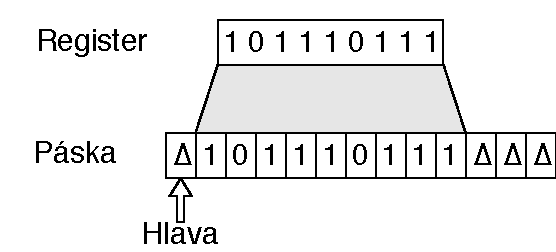
\includegraphics[scale=1]{img/register_to_tape.pdf}
    \caption{Ilustračný obrázok prevodu registra $x$ na pásku $TS$ $M_P$.}
    \label{fig:reg_to_tape}
\end{figure}

Potom, pre $TS$ $M_P$ je potreba inicializovať hlavu čo v našom prípade znamená, že posunieme hlavu $TS$ $M_P$ na \textit{least significant bit} (\textit{LSB}) t.j. na \textit{most right nonblank symbol} (najpravejší neblankový symbol) čo je realizovateľné $TS$. Táto inicializácia nášho $TS$ $M_P$ je nutná z toho dôvodu, že na začiatku máme celé nezáporné číslo ale neskôr sa môžeme dopracovať ku desatinným číslam kde je potreba vedieť kde je desatinná čiarka. V $TS$ $M_P$ budeme desatinnú čiarku reprezentovať tak, že pozícia hlavy ukazuje na \textit{LSB} čísla z čoho vieme, že desatinná bodka sa nachádza na pravej strane od tohto \textit{LSB} čísla. Proces inicializácie hlavy je ilustrovaný na obrázku \ref{fig:tape_init} v ktorom je hypotetická desatinná bodka znázornená červenou bodkou.\\

\begin{figure}[!h]
    \centering
    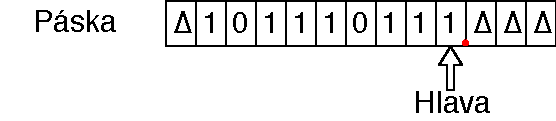
\includegraphics[scale=1]{img/tape_head.pdf}
    \caption{Ilustračný obrázok inicializácie hlavy $TS$ $M_P$ na páske.}
    \label{fig:tape_init}
\end{figure}

Predpokladajme, že zdrojový kód pre program $P$ v jazyku \textit{RationalC} má určitú formu kde každý jeden príkaz je zapísaný na osobitnom riadku kde všetky riadky sú očíslované od $0$ (pre prvý riadok) až po $N$ (posledný riadok).\\

Potom, pre každý jeden riadok, kde označíme číslo riadka ako $N$, vytvoríme jeden stav $q_N \in Q$ a pre každý príkaz na týchto riadokoch platí, že jednotlivé príkazy vieme previesť podľa nasledujúcich pravidiel.

\newpage
\begin{itemize}
    \item Príkaz $\texttt{if } x \ \% \ 2 == A$ \texttt{goto} $B$ kde $A = \{0, 1\}$ a $0 \leq B \leq N_{MAX}$ na riadku $N$\\[-1.5em]
        \begin{flushright}
        \begin{minipage}{0.90\textwidth}
            $TS$ $M_P$ bude obsahovať nasledujúce prechodové pravidlá pre tento príkaz
            \begin{center}
            \begin{tabular}{r@{ $=$ }l}
                $\delta(q_{N}, A)$       & $(q_{B}, A)$\\
                $\delta(q_{N}, \bar{A})$ & $(q_{N+1}, \bar{A})$
            \end{tabular}
            \end{center}
            kde $q_{B}, q_{N}, q_{N+1} \in Q$.\\

            Tento príkaz je možné chápať ako zmena stavu v $TS$ $M_P$ pričom sa hlava neposunie a ponechá sa pôvodný symbol pod pozíciou hlavy.
        \end{minipage}
        \end{flushright}
    \item Príkaz $x \texttt{ /= } 2$ na riadku $N$\\[-1.5em]
        \begin{flushright}
        \begin{minipage}{0.90\textwidth}
            $TS$ $M_P$ bude obsahovať nasledujúce prechodové pravidlá pre tento príkaz
            \begin{center}
            \begin{tabular}{r@{ $=$ }l}
                $\delta(q_{N}, 0)$ & $(q_{N+1}, L)$\\
                $\delta(q_{N}, 1)$ & $(q_{N+1}, L)$
            \end{tabular}
            \end{center}
            kde $q_{N}, q_{N+1} \in Q$.\\

            Tento príkaz je možné chápať ako posun hlavy $TS$ $M_P$ do ľava.
        \end{minipage}
        \end{flushright}
    \item Príkaz $x \texttt{ *= } 2$ na riadku $N$\\[-1.5em]
        \begin{flushright}
        \begin{minipage}{0.90\textwidth}
            $TS$ $M_P$ bude obsahovať nasledujúce prechodové pravidlá pre tento príkaz
            \begin{center}
            \begin{tabular}{r@{ $=$ }l}
                $\delta(q_{N}, 0)$ & $(q_{N+1}, R)$\\
                $\delta(q_{N}, 1)$ & $(q_{N+1}, R)$
            \end{tabular}
            \end{center}
            kde $q_{N}, q_{N+1} \in Q$.\\

            Tento príkaz je možné chápať ako posun hlavy $TS$ $M_P$ do prava.
        \end{minipage}
        \end{flushright}
    \item Príkaz \texttt{return} $0$ na riadku $N$\\[-1.5em]
        \begin{flushright}
        \begin{minipage}{0.90\textwidth}
            $TS$ $M_P$ bude obsahovať nasledujúce prechodové pravidlá pre tento príkaz
            \begin{center}
            \begin{tabular}{r@{ $=$ }l}
                $\delta(q_{N}, 0)$ & $(q_{reject}, 0)$\\
                $\delta(q_{N}, 1)$ & $(q_{reject}, 1)$
            \end{tabular}
            \end{center}
            kde $q_{N}, q_{reject} \in Q$ a $q_{reject} \in F$.\\

            Tento príkaz je možné chápať ako prechod $TS$ $M_P$ do koncového stavu ktorý je odmietajúci.
        \end{minipage}
        \end{flushright}
    \item Príkaz \texttt{return} $1$ na riadku $N$\\[-1.5em]
        \begin{flushright}
        \begin{minipage}{0.90\textwidth}
            $TS$ $M_P$ bude obsahovať nasledujúce prechodové pravidlá pre tento príkaz
            \begin{center}
            \begin{tabular}{r@{ $=$ }l}
                $\delta(q_{N}, 0)$ & $(q_{accept}, 0)$\\
                $\delta(q_{N}, 1)$ & $(q_{accept}, 1)$
            \end{tabular}
            \end{center}
            kde $q_{N}, q_{accept} \in Q$ a $q_{accept} \in F$.\\

            Tento príkaz je možné chápať ako prechod $TS$ $M_P$ do koncového stavu ktorý je akceptujúci.
        \end{minipage}
        \end{flushright}
\newpage
    \item Príkaz \texttt{odd}$(x)$ na riadku $N$\\[-1.5em]
        \begin{flushright}
        \begin{minipage}{0.90\textwidth}
            $TS$ $M_P$ bude obsahovať nasledujúce prechodové pravidlá pre tento príkaz
            \begin{center}
            \begin{tabular}{r@{ $=$ }l}
                $\delta(q_{N}, 0)$ & $(q_{N+1}, 1)$\\
                $\delta(q_{N}, 1)$ & $(q_{N+1}, 1)$
            \end{tabular}
            \end{center}
            kde $q_{N}, q_{N+1} \in Q$.\\

            Tento príkaz je možné chápať ako zápis symbolu $1$ na aktuálnej pozícii hlavy.
        \end{minipage}
        \end{flushright}
    \item Príkaz \texttt{even}$(x)$ na riadku $N$\\[-1.5em]
        \begin{flushright}
        \begin{minipage}{0.90\textwidth}
            $TS$ $M_P$ bude obsahovať nasledujúce prechodové pravidlá pre tento príkaz
            \begin{center}
            \begin{tabular}{r@{ $=$ }l}
                $\delta(q_{N}, 0)$ & $(q_{N+1}, 0)$\\
                $\delta(q_{N}, 1)$ & $(q_{N+1}, 0)$
            \end{tabular}
            \end{center}
            kde $q_{N}, q_{N+1} \in Q$.\\

            Tento príkaz je možné chápať ako zápis symbolu $0$ na aktuálnej pozícii hlavy.
        \end{minipage}
        \end{flushright}
\end{itemize}

Pri násobení a delení (pri použití príkazov $x \texttt{ /= } 2$ a $x \texttt{ *= } 2$) môže ale dôjsť ku tomu, že sa hlava dostane zo symbolu $0$ alebo $1$ na symbol blank. Môžu nastať dve možnosti a to keď sa hlava dostaneme na ľavý blank (prvý symbol pásky) alebo na pravý blank (blank za posledným znakom $0$ alebo $1$ ktorý je uložený na páske). Tieto prípady je potreba vyriešiť pričom môžu nastať iba vtedy, ak sme sa dostali na krajný (najpravejší alebo najľavejší) symbol $0$ alebo $1$ vedľa ktorého je z ľavej strany blank (pre najľavejší) alebo z pravej strany blank (pre najpravejší). Takže môžu nastať dva prípady.

\begin{itemize}
    \item Hlava je na najpravejšom symbole $0$ alebo $1$ a treba vykonať príkaz $x \texttt{ *= } 2$.\\[-1.5em]
        \begin{flushright}
        \begin{minipage}{0.90\textwidth}
            Príkladový prípad hlavy a pásky

            \begin{center}
                $\Delta 1 \red{\underbar{0}} \Delta \Delta \Delta \dots$
            \end{center}

            Po vykonaní príkazu $x \texttt{ *= } 2$ sa hlava dostane z najpravejšieho neblankového symbolu na pravý blankový symbol.

            \begin{center}
                $\Delta 1 0 \red{\underbar{$\Delta$}} \Delta \Delta \dots$
            \end{center}

            V hore uvedenom prípade by sme mali chybnú hodnotu čísla z toho dôvodu, že u nás pozícia hlavy určuje \textit{LSB} a tým pádom by sme mali nevalidné číslo keďže jeho \textit{LSB} by bol blankový symbol. Aby sme sa vyhli tejto situácii, pri každom posune doprava treba vykonať kontrolu zda tam je blankový symbol, ak tam je, tak ho prepíšeme na symbol $0$ a posunieme hlavu na tento symbol $0$, ak tam nie je, tak iba presunieme hlavu na ten symbol ktorým je $0$ alebo $1$.

            \begin{center}
                \begin{tabular}{l|l|c|c}
                    \multicolumn{1}{c|}{\textbf{Páska}} & \multicolumn{1}{c|}{\textbf{Hodnota}} & \multicolumn{1}{c|}{\textbf{Riadok}} & \multicolumn{1}{c}{\textbf{Nasledujúci príkaz}}\\
                    \hline
                    $\Delta \red{\underbar{1}} 0       \Delta \Delta \Delta \dots$ & $1$ & $n$   & $x \texttt{ *= } 2$\\
                    $\Delta 1 \red{\underbar{0}}       \Delta \Delta \Delta \dots$ & $2$ & $n+1$ & $x \texttt{ *= } 2$\\
                    $\Delta 1 0 \red{\underbar{$0$}}   \Delta \Delta \Delta \dots$ & $4$ & $n+2$ & $x \texttt{ *= } 2$\\
                    $\Delta 1 0 0 \red{\underbar{$0$}} \Delta \Delta \Delta \dots$ & $8$ & $n+3$ & $x \texttt{ *= } 2$\\
                \end{tabular}
            \end{center}

            V tabuľke stĺpec '\textit{páska}' zachytáva aktuálny stav pásky spolu s pozíciou hlavy čo je znázornené podčiarknutým červeným symbolom. Stĺpec '\textit{hodnota}' vyjadruje numerickú hodnotu ktorá sa nachádza na páske, '\textit{riadok}' udáva pozíciu v programe a '\textit{nasledujúci príkaz}' zobrazuje príkaz ktorý bude vykonaný.
        \end{minipage}
        \end{flushright}
    \item Hlava je na najľavejšom symbole $0$ alebo $1$ a treba vykonať príkaz $x \texttt{ /= } 2$.\\[-1.5em]
        \begin{flushright}
        \begin{minipage}{0.90\textwidth}
            Príkladový prípad hlavy a pásky

            \begin{center}
                $\Delta \red{\underbar{1}} 0 \Delta \Delta \Delta \dots$
            \end{center}

            Po vykonaní príkazu $x \texttt{ /= } 2$ sa hlava dostane z najľavejšieho neblankového symbolu na ľavý blankový symbol.

            \begin{center}
                $\red{\underbar{$\Delta$}} 1 0 \Delta \Delta \Delta \dots$
            \end{center}

            Ak by sme znovu vykonali tento príkaz, tak by došlo k abnormálnemu zastaveniu $TS$ $M_P$ pretože by nám spadla hlava. Tento prípad je možné riešiť tak, že ak sme na tomto ľavom blankovom symbole a treba vykonať príkaz pre posun do ľava t.j. vykonaným príkazom bude príkaz $x \texttt{ /= } 2$, tak sa celý obsah pásky posunieme o jeden symbol do prava (vykonáme $S_R$) a pred obsah pásky zapíšeme symbol $0$ pričom hlavu musíme vrátiť na pôvodné miesto -- na miesto ľavého blanku. Pre ilustráciu funkčnosti viz tabuľku dole.

            \begin{center}
                \begin{tabular}{l|l|c|c}
                    \multicolumn{1}{c|}{\textbf{Páska}} & \multicolumn{1}{c|}{\textbf{Hodnota}} & \multicolumn{1}{c|}{\textbf{Riadok}} & \multicolumn{1}{c}{\textbf{Nasledujúci príkaz}}\\
                    \hline
                    $\Delta 1 \red{\underbar{0}}       \Delta \Delta \Delta \dots$ & $2$     & $n$   & $x \texttt{ /= } 2$\\
                    $\Delta \red{\underbar{1}} 0       \Delta \Delta \Delta \dots$ & $1$     & $n+1$ & $x \texttt{ /= } 2$\\
                    $\red{\underbar{$\Delta$}} 1 0     \Delta \Delta \Delta \dots$ & $0.5$   & $n+2$ & $x \texttt{ /= } 2$\\
                    $\red{\underbar{$\Delta$}} 0 1 0   \Delta \Delta \Delta \dots$ & $0.25$  & $n+3$ & $x \texttt{ /= } 2$\\
                    $\red{\underbar{$\Delta$}} 0 0 1 0 \Delta \Delta \Delta \dots$ & $0.125$ & $n+4$ & $x \texttt{ /= } 2$\\
                \end{tabular}
            \end{center}

            V tabuľke stĺpec '\textit{páska}' zachytáva aktuálny stav pásky spolu s pozíciou hlavy čo je znázornené podčiarknutým červeným symbolom. Stĺpec '\textit{hodnota}' vyjadruje numerickú hodnotu ktorá sa nachádza na páske, '\textit{riadok}' udáva pozíciu v programe a '\textit{nasledujúci príkaz}' zobrazuje príkaz ktorý bude vykonaný.
        \end{minipage}
        \end{flushright}
\end{itemize}

Na základe tohto hore uvedeného popisu je možné zostrojiť pre program $P$ v jazyku $RationalC$ s počiatočnou hodnotou $x_0$ uloženou v registri $x$ ekvivalentný $TS$ $M_P$ a reťazec $w \in \{0,1\}^*$ tak, že $w \in L(M_P)$ práve vtedy keď program $P$ s počiatočnou hodnotou $x_0$ skončí s návratovou hodnotou $1$.

\newpage
\section{Literatúra} %#################################################################################

\bibliographystyle{slovakiso}
\begin{flushleft}
    \bibliography{quotation}
\end{flushleft}

\end{document}
